% Graph G and all possible spanning trees
\begin{figure}[htb]
\centering
\subfigure
{
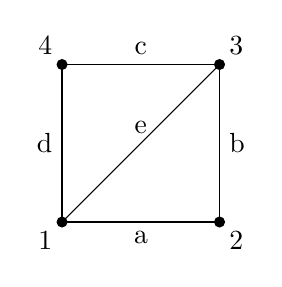
\begin{tikzpicture}[scale=2,baseline=(current bounding box.center)]

\node (n1) at (0,0) {};
\node (n2) at (1,0) {};
\node (n3) at (1,1) {};
\node (n4) at (0,1) {};

\draw (n1) node[anchor=north east] {$1$};
\draw (n2) node[anchor=north west] {$2$};
\draw (n3) node[anchor=south west] {$3$};
\draw (n4) node[anchor=south east] {$4$};

\foreach \i in {1,...,4}
{
	\fill (n\i) circle [radius=1pt];
};

\foreach \i/ \j/ \label/\position in {1/2/a/below, 2/3/b/right, 
					3/4/c/above, 4/1/d/left, 
					1/3/e/above}
{
	\path (n\i.center) edge node[\position] {\label} (n\j.center);
};
\end{tikzpicture}
}
\subfigure
{
	\begin{tabular}{cccc}
	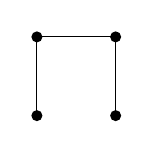
\begin{tikzpicture}

	\node (n1) at (0,0) {};
	\node (n2) at (1,0) {};
	\node (n3) at (1,1) {};
	\node (n4) at (0,1) {};

	\foreach \i in {1,...,4}
	{
		\fill (n\i) circle [radius=2pt];
	};

	\foreach \i / \j in {2/3, 3/4, 4/1}
	{
		\path (n\i.center) edge (n\j.center);
	};
	\end{tikzpicture}
	&
	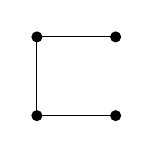
\begin{tikzpicture}

	\node (n1) at (0,0) {};
	\node (n2) at (1,0) {};
	\node (n3) at (1,1) {};
	\node (n4) at (0,1) {};

	\foreach \i in {1,...,4}
	{
		\fill (n\i) circle [radius=2pt];
	};

	\foreach \i / \j in {
	1/2, 
	%2/3, 
	3/4,
	4/1}
	{
		\path (n\i.center) edge (n\j.center);
	};
	\end{tikzpicture}
	&
	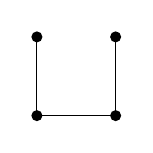
\begin{tikzpicture}

	\node (n1) at (0,0) {};
	\node (n2) at (1,0) {};
	\node (n3) at (1,1) {};
	\node (n4) at (0,1) {};

	\foreach \i in {1,...,4}
	{
		\fill (n\i) circle [radius=2pt];
	};

	\foreach \i / \j in {
	1/2, 
	2/3, 
	%3/4,
	4/1}
	{
		\path (n\i.center) edge (n\j.center);
	};
	\end{tikzpicture}
	&
	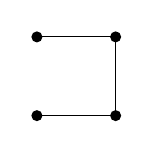
\begin{tikzpicture}

	\node (n1) at (0,0) {};
	\node (n2) at (1,0) {};
	\node (n3) at (1,1) {};
	\node (n4) at (0,1) {};

	\foreach \i in {1,...,4}
	{
		\fill (n\i) circle [radius=2pt];
	};

	\foreach \i / \j in {
	1/2, 
	2/3, 
	3/4}
	%4/1}
	{
		\path (n\i.center) edge (n\j.center);
	};
	\end{tikzpicture}
	\\
	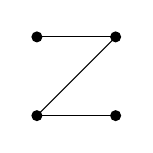
\begin{tikzpicture}

	\node (n1) at (0,0) {};
	\node (n2) at (1,0) {};
	\node (n3) at (1,1) {};
	\node (n4) at (0,1) {};

	\foreach \i in {1,...,4}
	{
		\fill (n\i) circle [radius=2pt];
	};
	\foreach \i / \j in {
	1/2, 
	%2/3, 
	3/4,
	%4/1,
	1/3}
	{
		\path (n\i.center) edge (n\j.center);
	};
	\end{tikzpicture}
	&
	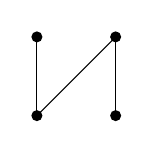
\begin{tikzpicture}

	\node (n1) at (0,0) {};
	\node (n2) at (1,0) {};
	\node (n3) at (1,1) {};
	\node (n4) at (0,1) {};

	\foreach \i in {1,...,4}
	{
		\fill (n\i) circle [radius=2pt];
	};
	\foreach \i / \j in {
	%1/2, 
	2/3, 
	%3/4,
	4/1,
	1/3}
	{
		\path (n\i.center) edge (n\j.center);
	};
	\end{tikzpicture}
	&
	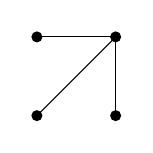
\begin{tikzpicture}

	\node (n1) at (0,0) {};
	\node (n2) at (1,0) {};
	\node (n3) at (1,1) {};
	\node (n4) at (0,1) {};

	\foreach \i in {1,...,4}
	{
		\fill (n\i) circle [radius=2pt];
	};
	\foreach \i / \j in {
	%1/2, 
	2/3, 
	3/4,
	%4/1,
	1/3}
	{
		\path (n\i.center) edge (n\j.center);
	};
	\end{tikzpicture}
	&
	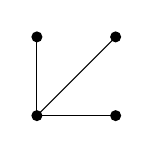
\begin{tikzpicture}

	\node (n1) at (0,0) {};
	\node (n2) at (1,0) {};
	\node (n3) at (1,1) {};
	\node (n4) at (0,1) {};

	\foreach \i in {1,...,4}
	{
		\fill (n\i) circle [radius=2pt];
	};
	\foreach \i / \j in {
	1/2, 
	%2/3, 
	%3/4,
	4/1,
	1/3}
	{
		\path (n\i.center) edge (n\j.center);
	};
	\end{tikzpicture}

	\end{tabular}
}
\caption{Graph $G$ and all its spanning trees}
\end{figure}



